% - Sicherheits-Applikation/ Spezielle Firewall
%    - Gefordert in diversen Compliance Richtlinien
% - was mach eine WAF im Prinzip?
%     - Zwischen Client und Server
%     - Analysiert Datenverkehr
% - Fokus auf web-Protokolle
%     - auf TCP/IP Layer 5
%     - HTTP, HTTPS, FTP
% - Traffic Analyse in Tiefe (Request & Response)
%     - HTTP (Kapitel 5.2) beschreibt diverse Angriffswege
%     - Erkennung anhand von Regeln
%         - Black- vs. whitelisting
%         - Vordefiniertes Regelwerk
\label{sec:waf-theory}
Ein \ac{waf} ist eine Sicherheits-Applikation, die in der Lage ist den Datenverkehr zu und von einer Webanwendung zu Analysieren.
Hierbei werden die übertragenen Inhalte in der Tiefe auf schädliche Inhalte überprüft.
Der in Abbildung \ref{fig:waf-porcess-flow} dargestellte Prozessablauf beschreibt wie eine \ac{waf} Nachrichten verarbeitet.

\begin{figure}[!hbt]
    \centering
    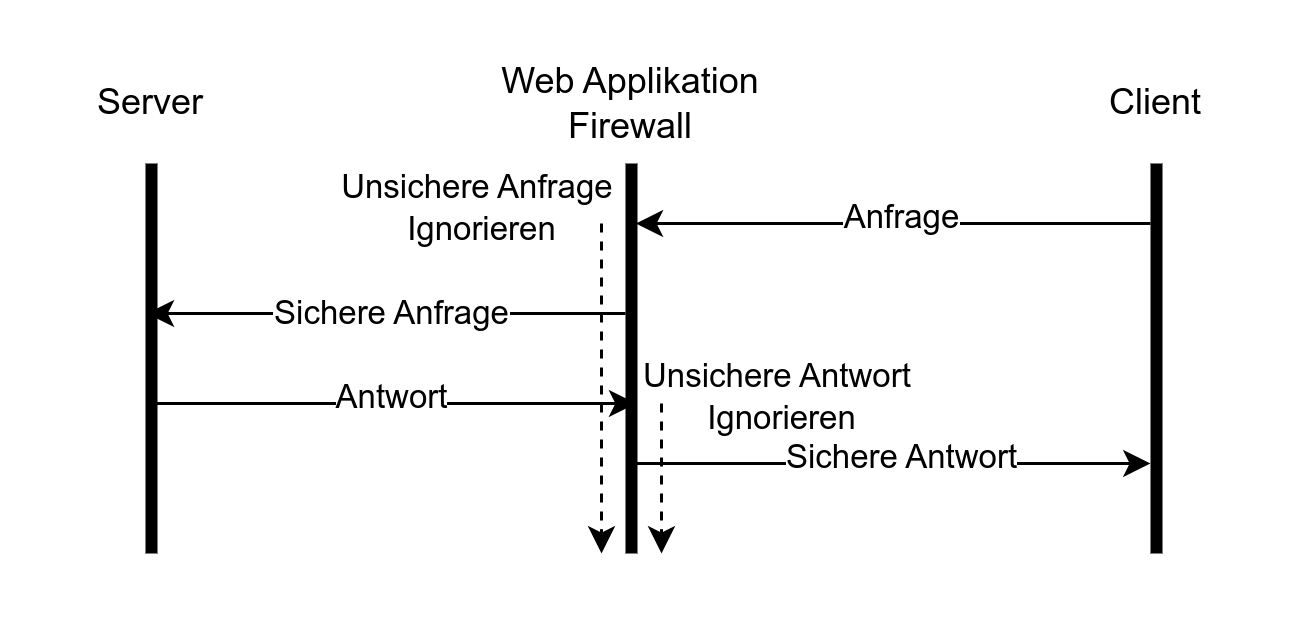
\includegraphics[width=0.9\textwidth]{./images/Waf-Process-fliow.png}
    \caption{Prozess Ablauf der Verarbeitung durch eine Web Application Firewall}
    \floatfoot{Quelle: In Anlehnung an \cite[S. 8]{guptaWEBAPPLICATIONFIREWALL2007}}
    \label{fig:waf-porcess-flow}
\end{figure}

Das grundlegende Muster ist, dass einen Nachricht an der \ac{waf} eintrifft und von dieser an den Server weitergegeben wird.
Dieser verarbeitet die Anfrage und sendet seine Antwort an die \ac{waf} die die Antwort an den Client weiterleitet.
Es besteht keine direkte Kommunikations-Verbindung zwischen Server und Client.
Die \ac{waf} ordnet der Anfrage die zugehörige Antwort zu.
Als schädlich erkannte Inhalte können sowohl in einer Anfrage als auch Antwort abgelehnt werden.
Anstatt einer abgelehnten Nachricht kann eine \ac{waf} auch eine eigene Antwort an den Client senden.
Das ermöglicht es Nutzern festzustellen, dass ein Fehler in seiner Anfrage oder der Konfiguration der \ac{waf} vorliegt.
Mittels einer ID, die der ersetzten Antwort angehängt wird lässt sich das Verhalten im Nachhinein nachvollziehen.
Neben den beiden Möglichkeiten \textit{weiterleiten} und \textit{ablehnen} kann eine \ac{waf} die in einer Anfrage erkannten schädlichen Inhalte auch neutralisieren und die Nachricht weitergeben\cite{schmitzGrundlagenWebApplication2018}.\\

Eine \ac{waf} wird in produktiven Umgebungen in einem Netzwerk \textit{vor} den zu schützenden Anwendungen positioniert.
Das heißt der geschützte Server befindet sich in einer \ac{dmz}.
Eine \ac{dmz} ist ein, von anderen Netzwerkaktivitäten abgeschnittenes Netzwerksegment, das nur durch die \ac{waf} sowie weitere Sicherheitsanwendungen zugänglich ist.
Dadurch soll verhindert werden, dass ein Nutzer auf anderem Weg als vorgesehen Zugriff auf den Server erhält.

Neben den \textit{on-premise} Deployment-Methoden, bei denen die \ac{waf} als \ac{vm} oder physischer Server im gleichen privaten Netzwerk wie die zu schützenden Server platziert ist, werden auch einige \ac{waf} als sogenannte \textit{Cloud-\ac{waf}} zur Verfügung gestellt.
Die \ac{waf} ist hier nicht im selben Netzwerk wie der Server sondern wird in einem fremden Netzwerk betrieben.
Die Daten fließen von der \ac{waf} durch das öffentliche Internet zu den zu sichernden Servern.
Dadurch ergeben sich einige Änderungen im Aufbau des Deployments:
Es muss sichergestellt werden, dass ein Client der eine Verbindung zum Server aufbauen möchte, bei der Namensauflösung (DNS) auf die \ac{waf} geleitet wird.
%% Ungenaue Vereinfachung
Der Server hingegen stellt sicher nur Verbindungen von der \ac{waf} zu akzeptieren.
Dies kann mit einer Firewall, die nur Verbindungen von der \ac{waf} akzeptiert, realisiert.
Es existieren auch Zertifikat basierte Verfahren, die die Authentizität der Datenherkunft sicherstellen.\\

% out of place

Eine Firewall\footnote{Wenn im folgenden von einer \textit{Firewall} gesprochen wird ist eine Firewall auf IP und Port Ebene gemeint. Eine Web Application Firewall wir immer mit \ac{waf} bezeichnet.} nimmt Filterung auf Internet- und Transportschicht (Layer 2 und 3) des TCP/IP Modells vor.
Operiert also hauptsächlich mit IP-Adresse und Port Nummer.
Eine \ac{waf} hingegen arbeitet auf der Anwendungsschicht (Layer4).
Der Fokus liegt auf Internet-Protokollen wie \ac{http} und \ac{https}. 
Aber auch Datentransferprotokolle wie FTP sind im Funktionsumfang einer \ac{waf}.

Da es sich bei \ac{http} und auch FTP um plaintext Protokolle handelt, bei denen der Datentransport in einer menschenlesbarer Form erfolgt, unterscheidet sich die Funktion einer \ac{waf} grundsätzlich von der einer Firewall.
Die Erkennung schädlicher Inhalte erfolgt aufgrund von Regeln, die Muster beschreiben die auf diese hindeuten.
In der Implementierung wird dies in der Regel durch die Verwendung regulärer Ausdrücke realisiert, diese bilden Muster ab die mit den Inhalten des Datenverkehrs abgeglichen werden.
Eine \ac{waf} muss jedes Datenpaket mit einer Anzahl von Regeln in der Größenordnung mehrerer hunderttausend bis Millionen Regeln abgleichen.
Der Rechenaufwand kann zwar durch optimierte Engines zur Auswertung regulärer Ausdrücke oder Tree-Pruning-Algorithmen die irrelevante Überprüfungspfade erkennen, verringert werden.
Jedoch ist der Rechenaufwand in einer \ac{waf} relativ hoch und die Hardware Anforderungen an eine \ac{waf} groß.
Auch muss bei einer vorgeschalteten \ac{waf} mit erhöhten Antwortzeiten gerechnet werden, die sich im Millisekunden Bereich befinden.

Da es im Aktuellen stand der Technik üblich ist Internet-Datenübertragung zu verschlüsseln, muss eine \ac{waf} in der Lage sein die verschlüsselte Kommunikation zu öffnen um so die Inhalte analysieren zu können. %% Nicht Öffnen Terminieren
Die SSL Verschlüsselung von \ac{https} wird also an der \ac{waf} terminiert.
Die Kommunikation zwischen Server \textit{hinter} der \ac{waf} und der \ac{waf} selber kann entweder unverschlüsselt oder mit einem separaten Satz Zertifikate erfolgen.
Die \ac{waf} verschlüsselt die Kommunikation nach der Verarbeitung wieder um sie an den Server weiterzugeben.
Die Abwägung ob in der \ac{dmz} verschlüsselt kommuniziert wird muss anhand von Compliance-Gesichtspunkten und der Vertrauenswürdigkeit der Umgebung erfolgen\cite{guptaWEBAPPLICATIONFIREWALL2007}.%% CLoud waf notwendig

\subsubsection{Verarbeitung einer Anfrage}
Der Zentrale Punkt, der in der der Thesis anhängenden Laborumgebung vermittelt werden soll, ist die Verarbeitung von Daten durch eine \ac{waf}.
In dem folgend Anschnitt wird beschreiben wie eine \ac{waf} konzeptionell implementiert ist um diese Aufgabe auszuführen.
Da die meisten Kommerziell erhältlichen \acp{waf} proprietäre Anwendungen sind, die keine Einsicht auf den Quellcode ermöglichen, basiert diese Beschreibung hauptsächlich auf der, als \textit{Open-Source} Anwendung vertriebenen \ac{waf}, \textit{ModSecurity}.
Da jedoch ein großer Teil der kommerziellen Anwendungen auf \textit{ModSecurity} aufbauen lässt sich eine gewisse Allgemeingültigkeit vermuten.

Die Verarbeitung in einer \ac{waf} erfolgt in vier Schritten. Der Fokus der Beschreibung liegt auf der Verarbeitung eines HTTP Requests.

Das folgende Kapitel basiert zu großen Teilen auf Artikel \cite{yuanResearchImplementationWEB2019}.

\paragraph{Request Parsing}
Das Request Parsing ist der erste Schritt nach dem Eintreffen einer Nachricht an einer \ac{waf}.
Vor diesem Schritt ist etwaige Verschlüsselung schon geöffnet, die Nachricht liegt in \ac{http}-Form vor.
Die Felder der \ac{http}-Nachricht werden nun ausgelesen und in ein Format überführt, das eine standardisierte Verarbeitung durch die \ac{waf} ermöglicht.
In dieser Form besteht jedoch immer noch eine gewisse Ambiguität in der Nachricht, die in einem Angriff genutzt werden könnte.
Deswegen muss einen Normalisierung der Felder erfolgen,
In Abbildung \ref{fig:norming} sind die Charakteristiken die normalisiert werden schematisch dargestellt.

\begin{figure}[!hbt]
    \centering
    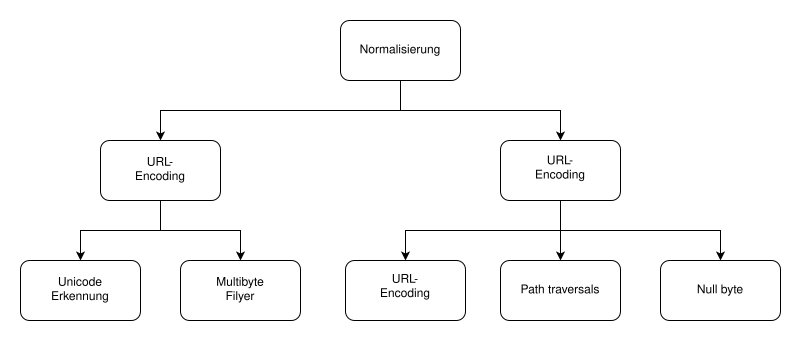
\includegraphics[width=0.9\textwidth]{./images/Normalisierung.png}
    \caption{Normalisierungsoperationen}
    \floatfoot{Quelle: In Anlehnung an \cite[S. 6]{guptaWEBAPPLICATIONFIREWALL2007}}
    \label{fig:norming}
\end{figure}

Normalisiert werden muss zum einen die Zeichendarstellung.
Die Nachricht muss in ein einheitliches Encoding überführt werden, außerdem müssen \textit{URL-Encodings} aufgelöst werden.
Hier werden Sonderzeichen mit drei Bytes dargestellt:
Das erste Zeichen ist immer ein \verb|%| gefolgt von einer Zahl in hexadezimaler Darstellung die das Zeichen repräsentiert.
Das \verb|@|-Zeichen wird von \verb|%40| repräsentiert.
Soll das Zeichen \verb|%| selber dargestellt werden muss dies mit \verb|%25| codiert werden.
Weitere Normalisierungsoperationen sind das Entfernen von \textit{Null Bytes}.
Ein \textit{Null Byte} ist kein darstellbares Zeichen, das aber jeh nach Umfeld Nebeneffekte haben kann.
Alle oben genannten Techniken können genutzt werden um nicht von regulären Ausdrücken erkannt werden zu können.

Eine weitere Gruppe von Normalisierungsoperationen sind Pfad-Normalisierungen.
Werden Pfade nicht normalisiert, kann ein Angreifer Zugriff auf Verzeichnisse erlangen, die nicht zugänglich sein sollten.

Ist der Request Parsing Schritt abgeschlossen, liegt einen Nachricht in einer Form vor, die eine einheitliche Analyse ermöglicht.

\paragraph{Muster-Abgleich gegen Regeln}
Die normalisierte Nachricht kann von der \ac{waf} nun auf schädliche Inhalte untersucht werden.
üblicherweise erfolgt dies durch den Abgleich gegen eine Regel.
Eine Solche besteht aus einem regulären Ausdruck und einem Set an Instruktionen wie mit der Nachricht, im Fall einer Übereinstimmung mit dem regulären Ausdruck, verfahren werden soll.
Es ist möglich, Nachrichten zu transformieren, beispielsweise können \ac{http}-Header hinzugefügt oder modifiziert werden.
Außerdem wird das weitere Verfahren definiert.

\begin{description}
    \item[reject] lehnt die Nachricht ab, es werden keine weiteren Überprüfungen durchgeführt und die Nachricht nicht weitergeleitet.
    Die \ac{waf} Antwort dem client mit einer vordefinierten Antwort, die das Schließen der Verbindung begründet.
    \item[drop] lehnt die Nachricht ab, es werden keine weiteren Überprüfungen durchgeführt und die Nachricht nicht weitergeleitet.
    Die \ac{waf} sendet dem Client keine Antwort und beendet die Kommunikation sofort.
    \item[pass] gibt die Nachricht weiter ohne weitere Überprüfungen durchzurühren.
    Ist eine Konfiguration nicht sorgfältig überprüft kann dies zu Einschränkungen in der Sicherheit einer \ac{waf} führen.
\end{description}

In den Operationen können auch weitere Matching-Operationen definiert werden an die die Nachricht weitergeleitet werden soll.
So kann die Menge an Regeln reduziert werden gegen die eine Nachricht überprüft werden muss.
Es wird ein Baum an Regeln aufgebaut und nur die für eine Nachricht relevanten Checks ausgeführt.
%So muss beispielsweise nur dann wenn der \ac{http}-Header der signalisiert, dass der \ac{http}-Body JSON formatiert ist, eine Überprüfung durchgeführt werden ob es sich um gültiges JSON handelt.
Es muss beispielsweise nur geprüft werden ob ein JSON-Objekt in einem \ac{http}-Body gültig ist, wenn der zu schützende Endpoint JSON erwartet.

Das Regelwerk einer \ac{waf} kann entweder durch \textit{White-} oder \textit{Blacklisting} erfolgen.
Whitelisting ermöglicht es genau zu kontrollieren welche Anfragen an einen Server gestellt werden könne.
Der daraus resultierende Konfigurationsaufwand für eine*n \ac{waf}-Consultant*in ist jedoch im Vergleich zu Blacklisting höher.
Blacklisting hingegen ermöglicht bei unsicherer Konfiguration, dass das Umgehen der \ac{waf} deutlich einfacher möglich ist.\\

Neben regelbasierter Erkennung schädlicher Inhalte bieten einige \acp{waf} Signatur basierte Verfahren an wie sie beispielsweise auch in einem Virenscanner genutzt werden.
Diese werden im Rahmen dieser Thesis jedoch nicht genauer betrachtet.

\paragraph{Logging}
Ein weiterer Schritt in der Verarbeitung einer Nachricht ist die Protokollierung, das sogenannte Logging.
Dies ist zur Nachvollziehbarkeit der Operation einer WAF wichtig und ermöglicht es die Qualität der Konfiguration der \ac{waf} zu beurteilen.
Aber auch nach einem erfolgreichen Angriff nachvollziehen wie dieser erfolgt ist und eventuell Schlüsse auf den Verursacher zuzulassen.

\paragraph{Weiteres Vorgehen}
Ist die Bearbeitung durch die \ac{waf} erfolgt, muss die Nachricht wieder in ein verständliches \ac{http} überführt werden.
Etwaige Änderungen an der Nachricht die durch die \ac{waf} durchgeführt werden müssen übernommen werden.
Des Weiteren muss etwaige Transportsicherheit auf dem Weg zum Ziel wieder angewendet werden.\\

Wird eine Nachricht abgelehnt, kann in deren Statt eine Antwort der \ac{waf} an den Client gesendet werden die ihn über den Vorgang informiert.
Beispielsweise kann eine \ac{http}-Nachricht mit einem 400er Status und der Information, dass der Client nicht die Berechtigung hat eine Aktion durchzuführen.



%\subsubsection{Erweiterte Funktionen}
%\paragraph{Lernen von Regeln aus vorhergegangenem Datenverkehr}
%\paragraph{KI-Features}
%\subsubsection{Deployment einer WAF}
%\paragraph{Postitionierung einer WAF}
%\paragraph{Betrieb einer WAF}
%\subsubsection{Schwächen und Nachteile einer WAF}
